\documentclass[a4paper,12pt]{article}

\usepackage[utf8]{inputenc}
\usepackage{polski}
\usepackage{fullpage}
\usepackage{hyperref}
\usepackage[pdftex]{graphicx} % Wsparcie dla obrazkow
\usepackage{listings}

\title{Wyznaczanie reprezentacji preferencji uniwersalych}
\author{Bartosz Górski \and Marcin Kaczyński \and Paweł Sokołowski}

\begin{document}

\maketitle

\section{Opis zadania} 

Szablon do wypełnienia. Jak ktoś chce napisać jakiś konkretny rozdział to niech się przy nim wpisze - może być w komentarzu. 
Jak nie to się później rozdzieli zadania.\\

Przykład wykorzystania bibliografii\cite{fst}. W bibliografii wpisy są z jakiegoś mojego wcześniejszego raportu, będą zmienione. Kompilacja:

\begin{itemize}
\item pdflatex raport (chyba musi być)
\item bibtex raport
\item pdflatex raport (x2)
\end{itemize}

Jak ktoś nie umie pisać w texie, to niech prześle plain text w notaniku.

\section{Założenia}
\section{Dane wejściowe i wyjściowe}
Dane wejściowe są przekazywane do aplikacji w postaci następujących plików:
\begin{itemize}
\item plik zawierający zbiór danych
\item plik z opisem relacji
\end{itemize}
Obsługiwanym formatem plików zawierających zbiór danych jest Csv. Wymagane jest aby w jednej z kolumn przechowywane były dane określające do której klasy należy dany wiersz. W drugim pliku znajduje się opis relacji pomiędzy klasami. \\
Dane wyjściowe wyświetlane są w polu tekstowym wewnątrz aplikacji. W każdej linii znajduje się opis jednego ze znalezionych minimalnych wzorców. Przykładowe wyjście programu:
\lstset{frame=single, xleftmargin=6pt, xrightmargin=6pt, framesep=6pt}
\begin{lstlisting}
1. (4#other meal) => (3#meal containing alcohol)
2. (2#non-vegetarian meal without pork, 
                  3#meal containing alcohol) => ()
3. (4#other meal, 3#meal containing alcohol) => ()
\end{lstlisting}
W nawiasach wymienione są opisy znalezionych atrybutów postaci: \{numer kolumny\}\#\{wartość atrybutu\}. Dane w lewym i prawym nawiasie przedstawiają atrybuty odpowiednio z lewego i prawego obiektu. 
\section{Szczegóły implementacji}

Implementacja została przygotowana w języku C\# i działa na platformie .NET Framework 4.0. Implementacja związana z algorytmem została podzielona na 4 projekty: Algorithm, DAL, HashTree i pomocniczy projekt Common.\\

W projekcie Algorithm znajdują się wszystkie klasy i interfejsy w bezpośredni sposób związane z interfejsem. Projekt DAL zawiera implementacje dostępu do danych, a więc w tym przypadku parsowanie plików z danymi do postaci wykorzystywanej w algorytmie. W projekcie HashTree znalajdują się interfejsy i implementacja drzewa mieszającego. Projekt Common zawiera wspólne klasy wykorzystywane w pozostałych projektach. W projekcie Common znajdują się niemal jedynie obiekty DTO. Obiekty te same w sobie nie wykonują operacji, dlatego nie będą szczegółowo opisywane.\\

W celu zapewnienia elastyczności skorzystano w projekie ze wzorca Dependency Injection. Zgodnie z wzorcem, na implementację algorytmu składa się szereg interfejsów, których odpowiedzialności przestawiaja się następująco:\\

Za główny interfejs można uznać \textit{IAlgorithm}, a jego podstawowym zadaniem jest znajdowanie preferencji uniwersalnych. Interfejs jest implementowany przez klasy \textit{Generators} i \textit{ModifiedApriori}. Podstawowa różnica pomiędzy klasami polega na tym, że klasa Generators do obliczania minimalnych preferencji wykorzystuje informację o generatorach do odrzucania większej liczby zbiorów kandydujących. Obie implementacje operują na wierszach
typu \textit{Row}/\textit{SimpleRow}, które są odwzorowaniem danych w postaci wygodnej do prowadzenia obliczeń. Do znajdywania zbiorów kandydujących wykorzystywany jest interfejs \textit{ICandidatesGenerator}. Za znajdowanie podzbiorów wspieranych w transakcjach odpowiada \textit{IHashTree}. Wczytywanie danych odbywa się za pomocą \textit{IDataManager}, a konwersja wyników do postaci wygodnej dla użytkownika za pomocą \textit{IResultsConverter}.\\

Ogólnie przebieg działania całego algorytmu składa się z następujących kroków:

\begin{enumerate}
\item wczytanie i parsowanie danych,
\item wykonanie obliczeń,
\item parsowanie wyników do czytelnej postaci
\end{enumerate}

Wykonanie obliczeń (2) przebiega wg następującego schematu:\\

W kolejnych iteracjach znajdywane są nowe zbiory kandydujące, dla wszystkich zbiorów obliczane są dwa liczniki mówiące o tym jakie wsparcie mają te zbiory w klasie transakcji spełniających i nie spełniających relację. Aby zapewnić wydajne obliczanie wartości omawianych liczników, wykorzystywane jest drzewo mieszające tworzone w każdej iteracji dla zbioru kandydatów. Po obliczeniu liczników podejmowana jest decyzja o tym, czy dany kandydat
jest minimalnym wzorcem, czy należy go odrzucić lub analizować dalej. Na tym etapie (opcjonalnie) podejmowana jest decyzja czy któryś z podzbiorów danego zbioru kandydującego jest generatorem. Jeżeli tak, taki zbiór nie będzie analizowany dalej.

\section{Wyniki}

\subsection{Wyniki podstawowe}

Tutaj będzie opis wyników dla danych z artykułu.

\subsection{Wyniki dla złożonych danych}

A tutaj wyniki dla normalnych danych. Na pewno musi być zbiór z samochodami, ten który był na którymś lab.

\section{Wnioski}

\appendix
\section{Podręcznik użytkownika}

Do uruchomienia aplikacji wymagany jest zainstalowany .NET Framework 4.0. Nie jest konieczna instalacja dodatkowych programów, bibliotek lub komponentów.\\

Do obsługi algorytmu został przygotowany prosty graficzny interfejs, opierający
się na idei instalatora. W kolejnych krokach użytkownik wybiera kolejne dopuszczalne opcje i zatwierdza je klikając przycisk Next. Możliwe jest cofnięcie się do poprzedniego widoku za pomocą przycisku Prev. Kolejne widoki wyglądają następująco:

\begin{figure}[h!]
\begin{center}
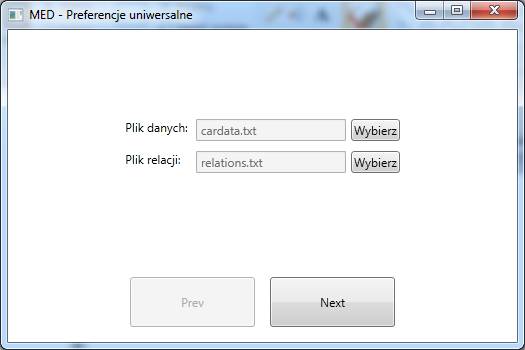
\includegraphics[width=\textwidth]{img/1.png}
\caption{Wybór plików z danymi}
\label{krok1}
\end{center}
\end{figure}

W kroku pierwszym\ref{krok1} należy wbrać pliki z danymi, klikając w przyciski Wybierz. Pliki wybiera się wykorzystując standardowy dialog wyboru plików z systemu Windows. Nie ma ograniczenia na rozszerzenie pliku.\\

Plik z danymi powinien być poprawnym pod względem budowy plikiem csv. W pliku powinny być kolejne wiersze w których w każdym znajduje się taka sama liczba kolumn oddzielonych określonym separatorem.\\

Plik z relacjami składa się z wielu linii. W każdej z nich znajduje się wpis postaci:
\lstset{frame=single, xleftmargin=6pt, xrightmargin=6pt, framesep=6pt}
\begin{lstlisting}
a<b
\end{lstlisting}
Oznacza to, że klasa {\bf a} jest w ralacji z klasą {\bf b}.
Dla przykładowego grafu relacji (\ref{relat}) plik powinien być postaci:
\lstset{frame=single, xleftmargin=6pt, xrightmargin=6pt, framesep=6pt}
\begin{lstlisting}
Y<V
Z<V
X<Y
X<Z
U<W
\end{lstlisting}

\begin{figure}[h!]
\begin{center}
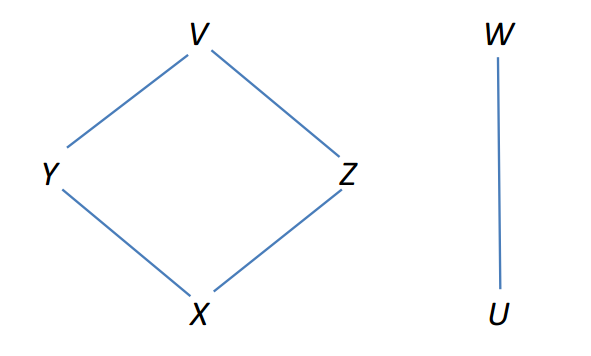
\includegraphics[width=\textwidth]{img/relations.png}
\caption{Przykładowy graf relacji}
\label{relat}
\end{center}
\end{figure}


\begin{figure}[h!]
\begin{center}
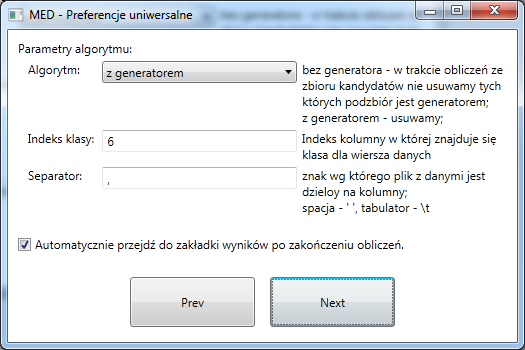
\includegraphics[width=\textwidth]{img/2.png}
\caption{Wybór parametrów}
\label{krok2}
\end{center}
\end{figure}

W kroku drugim\ref{krok2} należy wybrać parametry algorytmu. Dopuszczono wybór samego algorytmu - możliwe jest wykonanie algorytmu w wersji wykorzystującej oraz nie wykorzystującej faktu o podzbiorach będących generatorami.\\

W tym kroku należy również wybrać separator wykorzystywany w pliku danych, oraz określić indeks kolumny która zawiera klasę do której przypisany jest dany wiersz.\\

\begin{figure}[h!]
\begin{center}
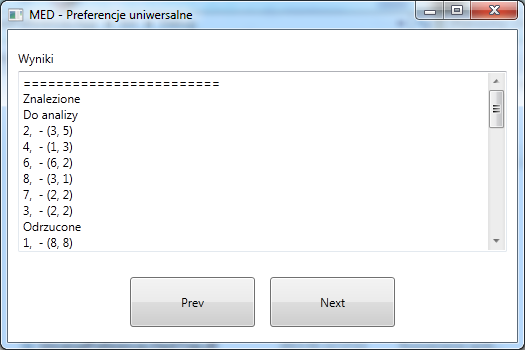
\includegraphics[width=\textwidth]{img/3.png}
\caption{Widok obliczeń}
\label{krok3}
\end{center}
\end{figure}

Krok trzeci\ref{krok3} to widok prezentowany w trakcie wykonywania obliczeń. W widoku wyświetlane są informacje diagnostyczne mówiące o tym które zbiory kandydujące zostały uznane za minimalne wzorce kontrastowe, które zostały odrzucone a które zostaną poddane dalszej analizie. Jeżeli w poprzednim kroku zaznaczono opcję Automatycznie przejdź do zakładki wyników po zakończeniu obliczeń, to po znalezieniu wszystkich wzorców program wyświetli widok wyników\ref{krok4}.\\

\begin{figure}[h!]
\begin{center}
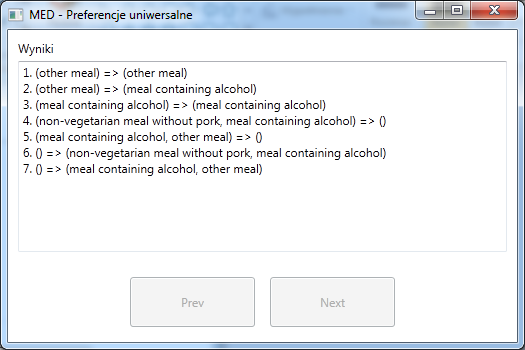
\includegraphics[width=\textwidth]{img/4.png}
\caption{Widok wyników}
\label{krok4}
\end{center}
\end{figure}

\bibliographystyle{plain}
\bibliography{bibliografia}

\end{document}
